% -------------------------------------------------------------------------------- %

\begin{exercise}[Exercise 8.1]

The nonplanning method looks particularly poor in Figure \ref{fig:8.3} because it is a one-step method;
a method using multi-step bootstrapping would do better.
Do you think one of the multi-step bootstrapping methods from Chapter 7 could do as well as the Dyna method?
Explain why or why not.

\setcounter{section}{8}
\setcounter{figure}{2}

\begin{figure}[H]
    \centering
    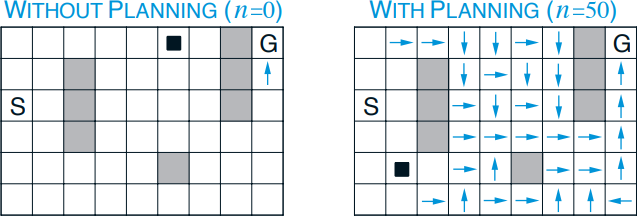
\includegraphics[width = 0.5 \textwidth]{4.45.png}
    \caption
    {
        Policies found by planning and nonplanning Dyna-Q agents halfway through the second episode.
        The arrows indicate the greedy action in each state;
        if no arrow is shown for a state, then all of its action values were equal.
        The black square indicates the location of the agent.
    }
    \label{fig:8.3}
\end{figure}

\end{exercise}

% -------------------------------------------------------------------------------- %

\begin{solution}

Judging by the previous exercside: No!

In each time step of an episode

\begin{itemize}
    \item an $n$-step Dyna method performs $n$ one-step updates (i.e. looks one step into the future $n$ times), while
    \item an $m$-step bootstrapping method performs a single $m$-step update (i.e. looks $m$ steps into the future one time).
\end{itemize}

The former thus aquires an accurate approximation of only a few state(-action) values, like hedgehogs (click \href{https://mathwithbaddrawings.com/2019/10/30/the-fox-hedgehog-game/}{here}).
The latter, on the other hand, aquires an inaccurate approximation of a large number state(-action) values, like foxes.

Apparently, in this context, it is more beneficial, to be a fox.

\end{solution}

% -------------------------------------------------------------------------------- %
